\documentclass{jarticle}

\usepackage{tam}
\usepackage{fleqn}
\usepackage{url}
\usepackage{bm}
\usepackage[dvipdfmx]{graphicx}
\usepackage[dvipdfmx]{color}
%\usepackage{color}
\usepackage{colordef}
\usepackage{amssymb}
\usepackage{pdfpages}
\usepackage{amsmath}

%%%%%%%%%% Command alias %%%%%%%%%%
\newcommand{\IB}{$\bullet$}
\newcommand{\IC}{$\circ$}
\newcommand{\IS}{$*$}
%%%%%%%%%%%%%%%%%%%%%%%%%%%%%%%%%%%

\title{電力運用最適化問題における動的計画法による求解}
\author{神戸大学大学院 奥村侑真}
\date{}

\def\baselinestretch{1.02}
\renewcommand{\thefootnote}{\roman{footnote}}

\begin{document}
\maketitle

\section{はじめに}
図\ref{fig:tecseed1}に示す電力ネットワークに対する，電力クラスタの電力運
用最適化モデルを示す．

\begin{figure}[h]
 \centering
 
\includegraphics[width=155mm]{../tecseed.pdf}
 \caption{テクシード構成図}
 \label{fig:tecseed1}
\end{figure}

\section{準備}

基本要素およびそのスペックを表す定数(\IB を付して記す)と状態変数(\IC を付
して表す)として以下のものを用意する．

%\begin{itemize}
% \item[$\triangleright$] 電力クラスタC$_{i}$ $(i=1,\ldots,N)$:
\begin{itemize}
 \item[\IS] 期T$_k$ ($k=1,\ldots,K$)．本検証では各期の幅は$60$秒としている．
 \item[\IS] 太陽光発電機G
 \item[\IS] 消費機器D$^{\rm A}$
 \item[\IS] 消費機器D$^{\rm B}$
 \item[\IS] 消費機器D$^{\rm C}$
 \item[\IS] 固定バッテリーB$^{\rm F}$
  \begin{itemize}
   \item[\IB] 固定バッテリーの容量 $\overline{b}$
  \end{itemize}
 \item[\IS] 電力変換器(太陽光) E$^{\rm P}$
  \begin{itemize}
   \item[\IB] 変換効率 $\alpha^{\rm P}$

  \end{itemize}
 \item[\IS] 電力変換器(系統電力) E$^{\rm S}$
 \item[\IS] 電力変換器(消費機器A) E$^{\rm A}$
  \begin{itemize}
   \item[\IB] 変換効率 $\alpha^{\rm DA}$
  \end{itemize}
 \item[\IS] 電力変換器(消費機器B) E$^{\rm B}$
  \begin{itemize}
   \item[\IB] 変換効率 $\alpha^{\rm DB}$
  \end{itemize}
 \item[\IS] 電力変換器(消費機器C) E$^{\rm C}$
  \begin{itemize}
   \item[\IB] 変換効率 $\alpha^{\rm DC}$
  \end{itemize}
 \item[\IS] 電力変換器(固定バッテリー)E$^{\rm BF}$
  \begin{itemize}
   \item[\IB] 充電効率 $\alpha^{\rm FC}$
   \item[\IB] 放電効率 $\alpha^{\rm FD}$
   %\item[\IB] 自己放電効率 $\alpha^{\rm FT}$
  \item[\IB] 単位時間あたりの最大充電電量 $a^{\rm FC}$
  \item[\IB] 単位時間あたりの最大充放電量 $a^{\rm FD}$
  \end{itemize}
 \item[\IS] 系統電力S
   \begin{itemize}
   \item[\IB] 系統買電単価 $p^{\rm BY}_{k}$
   \item[\IB] 単位時間あたりの最大系統買電量 $a^{\rm BY}$
   \item[\IB] 系統売電単価 $p^{\rm SL}_{k}$
   \item[\IB] 単位時間あたりの最大系統売電量 $a^{\rm SL}_{k}$
  \end{itemize}
\end{itemize}

\section{定数・変数 \mbox{\normalsize\rm 
~ (定数を「\IB」，変数を「\IC」を付して記すものとする)}}

 \begin{itemize}
  \item[\IB] 太陽光発電電力量(変換前) $g^{\rm P1}_{k}$
  \item[\IC] 太陽光発電電力量(変換後) $g^{\rm P2}_{k}$
  %\item[\IC] ムダ電力量 (太陽光発電出力抑制量)$v_{k}$ \\[-2.5ex]
  %
  \item[\IC] 消費電力A (変換前) $d^{\rm A1}_{k}$
 \item[\IB] 消費電力A (変換後) $d^{\rm A2}_{k}$
  %
  \item[\IC] 消費電力B (変換前) $d^{\rm B1}_{k}$
  \item[\IB] 消費電力B (変換後) $d^{\rm B2}_{k}$
  %
 \item[\IC] 消費電力C (変換前) $d^{\rm C1}_{k}$
  \item[\IB] 消費電力C (変換後) $d^{\rm C2}_{k}$
  %
  \item[\IB] 固定バッテリーのSOCの初期段階 $i_{0}$
  \item[\IB] 固定バッテリーのSOCを離散化したときの分割数$B$
  \item[\IC] 固定バッテリーの期末のSOC $b^{\rm F}_{k}$
  \item[\IC] 状態 $s_{i}(\in S_{k-1})$から$ s_{j} (\in S_{k})$へ遷移するときの固定バッテリーの充電量(変換前) $x^{\rm FC1}_{k}(s_{i},s_{j})$
  \\ただし，$x^{\rm FC1}_{k}(s_{i},s_{j}) < 0$を満たしているときは$|x^{\rm FC1}_{k}(s_{i},s_{j})|$だけ放電を行っていると解釈する．
  \item[\IC] 状態 $s_{i}(\in S_{k-1})$から$ s_{j} (\in S_{k})$へ遷移するときの固定バッテリーの充電量(変換後) $x^{\rm FC2}_{k}(s_{i},s_{j})$
   \\ただし，$x^{\rm FC2}_{k}(s_{i},s_{j}) < 0$を満たしているときは$|x^{\rm FC2}_{k}(s_{i},s_{j})|$だけ放電を行っていると解釈する．
  %\item[\IC] 固定バッテリーの放電量(変換前) $x^{\rm FD1}_{k}$
  %\item[\IC] 固定バッテリーの放電量(変換後) $x^{\rm FD2}_{k}$ \\[-2.5ex]

  %
  \item[\IC] 状態 $s_{i}(\in S_{k-1})$から$ s_{j} (\in S_{k})$へ遷移するときの系統買電力量$s^{\rm BY}_{k}(s_{i},s_{j})$  \\ただし，$s^{\rm BY}_{k}(s_{i},s_{j})< 0$を満たしているときは$|s^{\rm BY}_{k}(s_{i},s_{j}) |$だけ系統に売電を行っていると解釈する．
  %\item[\IC] 系統売電力量$s^{\rm SL}_{k}$
  
  %\item[\IC] 系統電力量(変換前)$s^{1}_{k}$．
  %\item[\IC] 系統電力量(変換後)$s^{2}_{k}$．
  %\item[\IB] 変換効率$\alpha^{\rm S}$．
  %
\end{itemize}


\section{動的計画法によるアプローチ}
この節では，前節で示した定数・変数を用いて，電力運用最適化問題に対して動的計画法によるアプローチでの求解方法を述べる．
なお，本問題で現れる定数・変数と電力クラスタとの関係を図\ref{fig:tecseed}に示す．
\subsection{定式化}
まず，バッテリーのSOCとしてとりうる値を，0が最小値となり $\overline{b}$が最大値となるように，等間隔に $B( \geq 2)$段階で離散化する．これにより，期 \(k\) の末尾におけるSOCは以下の \(B\) 個の値のいずれかをとる：
\[
0,\ \frac{1}{B-1}\overline{b},\ \frac{2}{B-1}\overline{b},\ \dots,\ \overline{b}．
\]
便宜上，期 $k$ の末尾においてバッテリーのSOCが $\frac{i}{B-1}\overline{b}$である状態を，「バッテリーのSOCが $i$ 段階である」と呼ぶことにする$(i=0,1,\dots ,  B - 1)$．

次に，状態を要素に持つ集合$S_{0},S_{1},\dots,S_{K-1}$を以下のように定義する：
\begin{equation}
S_k = \begin{cases}
  \left\{  s_{i_0}  \right\} ,\quad \text{if } k = 0 \\
  \left\{ s_{i} \mid i = 0, 1, \dots, B - 1 \right\} ,\quad \text{if } 1 \leq k \leq K．
\end{cases}
 \label{eq:state}
\end{equation}

ここで，状態$s_{i}( \in S_{k})$ は，期 $k$の末尾におけるバッテリーのSOCが$i$段階である状態を表す．


状態 $s_{i}(\in S_{k-1})$から$ s_{j} (\in S_{k})$への遷移に伴う評価関数を$w_{k-1}(s_{i},s_{j})$とする．ただし，問題を解くための時間的計算量を小さくるために，系統から買う電力量が$-a^{\rm SL}$以上かつ$a^{\rm BY}$以下であるような状態遷移のみを認めることにする．状態遷移のイメージを図\ref{fig:network}に示す．このとき，問題は以下のように定式化できる．

\begin{figure}[h]
 \centering
 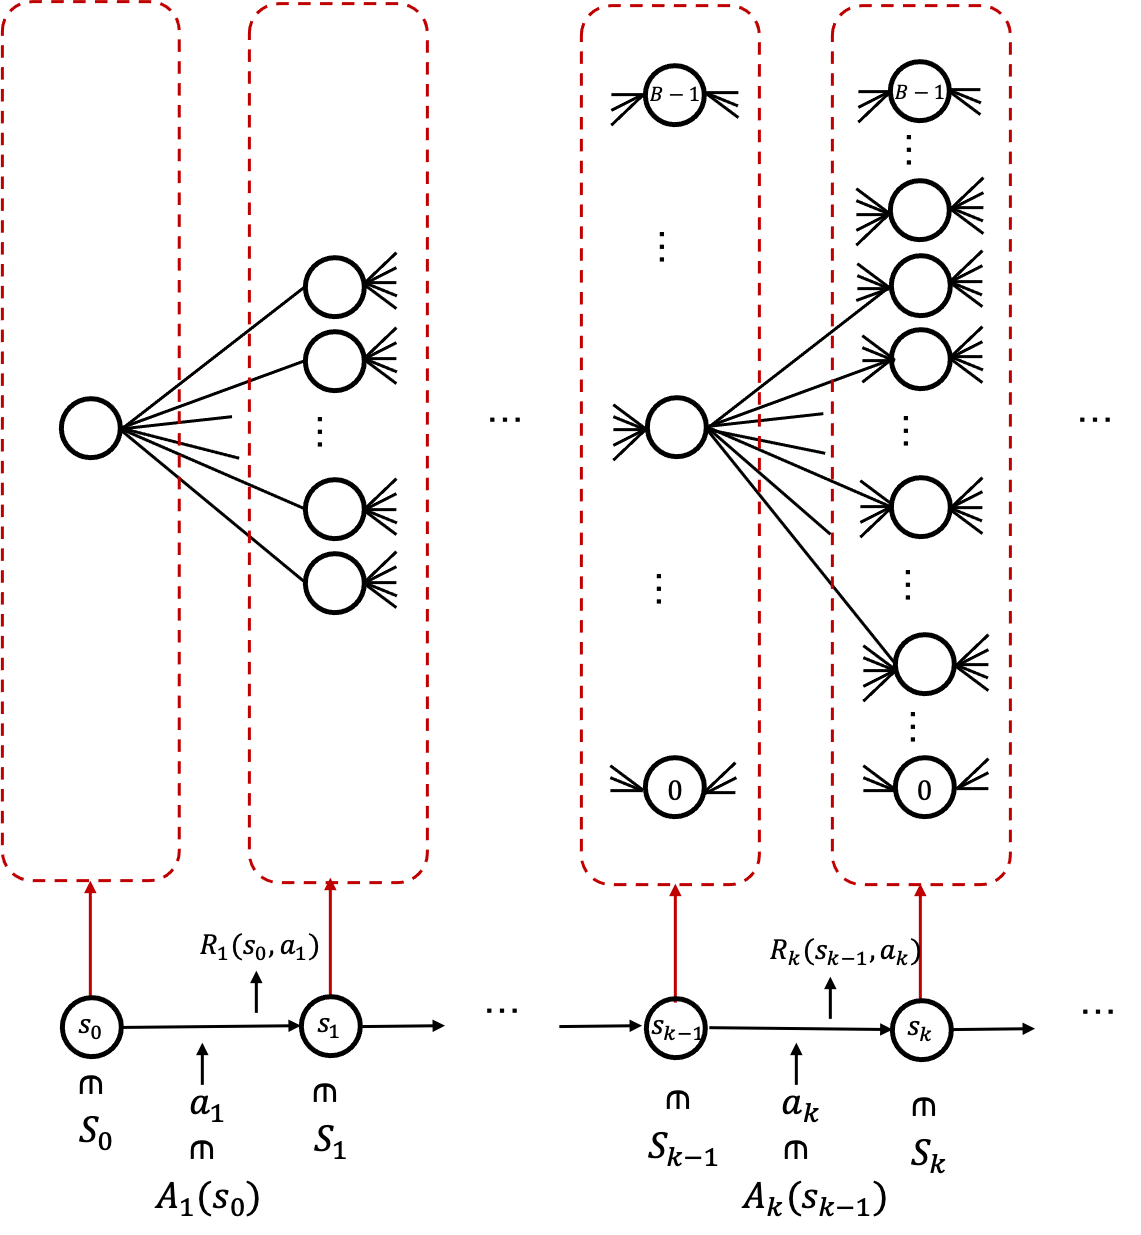
\includegraphics[width=145mm]{../figure/network.png}
 \caption{状態遷移のイメージ}
 \label{fig:network}
\end{figure}



\begin{equation}
    \text{Minimize} \quad \{ \sum_{k=0}^{K-1} w_k(s_i,s_j) | s_i \in S_k, s_j \in S_{k+1}, -a^{\rm SL}  \leq  \frac{j - i}{B-1}\overline{b} \leq a^{\rm BY} \}
 \label{eq:minimize}
\end{equation}


以下，評価関数の計算方法について述べる．工場を管理する人目線で考えると，お金の減少量をなるべく抑えることが望ましいと考えられる．そのことに留意すると，評価関数 $w_{k-1}(s_{i},s_{j})$の表し方のひとつとして以下のようなものが考えられる：
\begin{equation}
  %w_{k-1}(s_{i},s_{j}) = p_k^{\rm BY/SL} \left[ \frac{j - i}{n-1} \cdot \overline{b} - \{ g_k^{\rm P2} - (d_k^{\rm A2} + d_k^{\rm B2} + d_k^{\rm C2}) \} \right]．
  w_{k-1}(s_{i},s_{j}) = \begin{cases}
   p_k^{\rm BY}s_k^{\rm BY}(s_{i},s_{j}) ，  \text{if }  s_k^{\rm BY}(s_{i},s_{j}) \geq 0\\
   p_k^{\rm SL}s_k^{\rm BY}(s_{i},s_{j}) ，\text{otherwise}．
   \end{cases}
 \label{eq:weight}
\end{equation}


ここで， 電力の収支を考慮すると，
\begin{equation}
 s_k^{\rm BY}(s_{i},s_{j})= 
 d_k^{\rm A1}+ d_k^{\rm B1} + d_k^{\rm C1}+  x_k^{\rm FC1}(s_{i},s_{j}) - g_k^{\rm P2}\\
  \label{eq:pass_abst}
\end{equation}

が成り立つので，
\begin{equation}
 s_k^{\rm BY}(s_{i},s_{j}) = \begin{cases}
 \frac{d_k^{\rm A2}}{\alpha^{\rm DA}} + \frac{ d_k^{\rm B2}}{\alpha^{\rm DB}} + \frac{ d_k^{\rm C2}}{\alpha^{\rm DC}}+  \frac{x_k^{\rm FC2}(s_{i},s_{j})}{\alpha^{\rm FC}} - \alpha^{\rm P}  g_k^{\rm P1} ，\text{if}(x_k^{\rm FC2}(s_{i},s_{j}) \geq 0) \\
 
  \frac{d_k^{\rm A2}}{\alpha^{\rm DA}} + \frac{ d_k^{\rm B2}}{\alpha^{\rm DB}} + \frac{ d_k^{\rm C2}}{\alpha^{\rm DC}}+  \alpha^{\rm FD}x_k^{\rm FC2}(s_{i},s_{j}) - \alpha^{\rm P}  g_k^{\rm P1}，\text{otherwise}
 
 \end{cases}
 \label{eq:pass}
\end{equation}
が成立する．また，ある期の末からその1期次の期の末までのバッテリーの変化量に注目すると，

\begin{equation}
 x_k^{\rm FC2}(s_{i},s_{j}) =  \frac{j - i}{B-1} \overline{b}
 \label{eq:BF}
\end{equation}
となるので，(\ref{eq:pass})，(\ref{eq:BF})より，

\begin{equation}
 s_k^{\rm BY}(s_{i},s_{j}) = \begin{cases}
 \frac{d_k^{\rm A2}}{\alpha^{\rm DA}} + \frac{ d_k^{\rm B2}}{\alpha^{\rm DB}} + \frac{ d_k^{\rm C2}}{\alpha^{\rm DC}}+  \frac{1}{\alpha^{\rm FC}}\frac{j - i}{B-1} \overline{b} - \alpha^{\rm P}  g_k^{\rm P1} ，\text{if}(\frac{j - i}{B-1} \overline{b} \geq 0) \\
 
  \frac{d_k^{\rm A2}}{\alpha^{\rm DA}} + \frac{ d_k^{\rm B2}}{\alpha^{\rm DB}} + \frac{ d_k^{\rm C2}}{\alpha^{\rm DC}}+  \alpha^{\rm FD}\frac{j - i}{B-1} \overline{b} - \alpha^{\rm P}  g_k^{\rm P1} ，\text{otherwise}
 
 \end{cases}
 \label{eq:SBY}
\end{equation}
がいえる．(\ref{eq:SBY})の右辺に現れる全ての文字は既知であるため，(\ref{eq:weight})の右辺に現れる全ての文字は既知となる．よって，任意の$i,j,k(0\leq k \leq K)$について，状態 $s_{i}(\in S_{k-1})$から$ s_{j} (\in S_{k})$への遷移に伴う評価関数$w_{k-1}(s_{i},s_{j})$を設定することができる．


\begin{figure}[h]
 \centering
 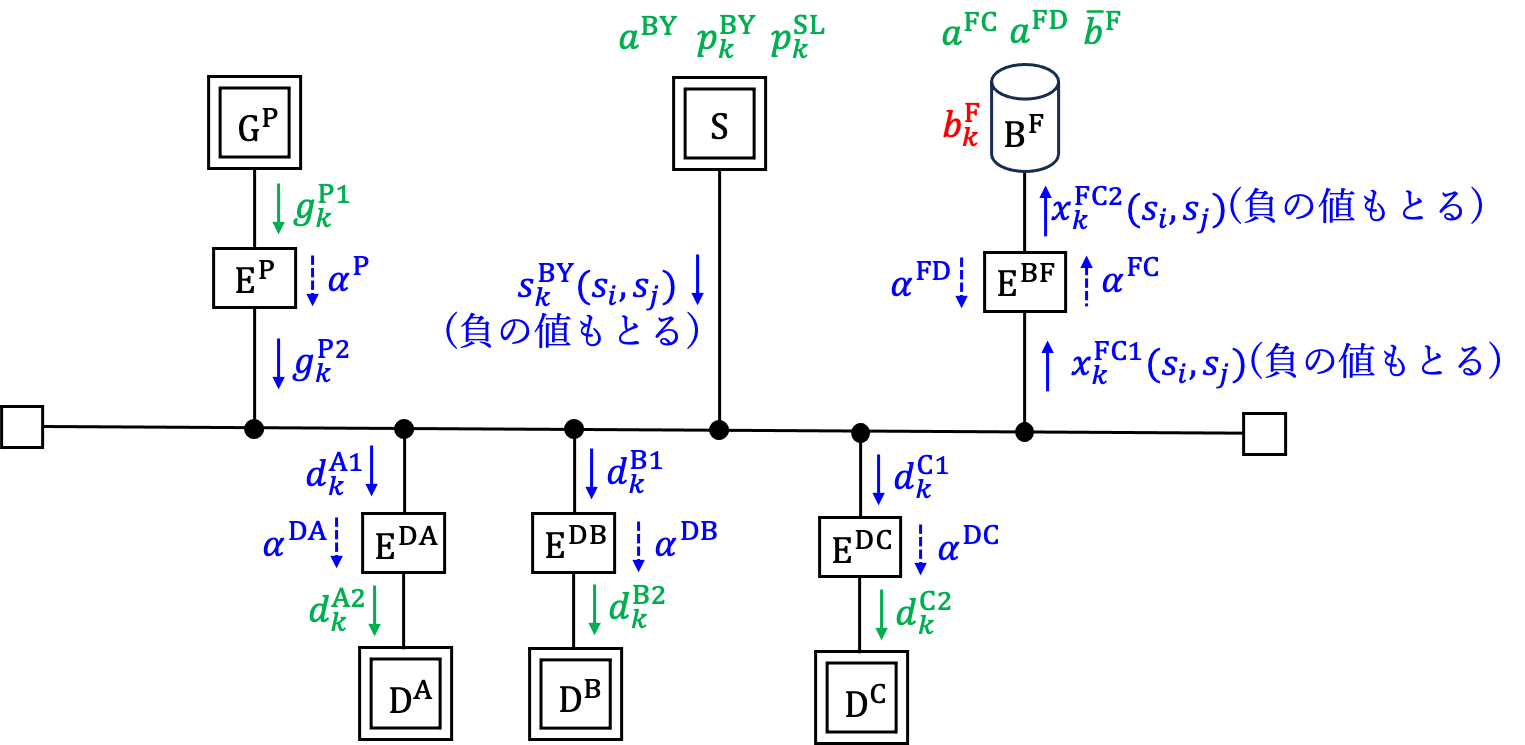
\includegraphics[width=140mm]{../figure/tecseed20251022.png}
 \caption{電力クラスタの構成図 (\textcolor{red}{赤: 決定変数}，\textcolor{blue}{青: 従属変数}，\textcolor{green3}{定数(外生変数)})}
 \label{fig:tecseed}
\end{figure}

\subsection{最適性の原理と更新式}
本問題は，”最適経路の部分経路もまた最適でなければならない”という最適性の原理を満たしており，動的計画法により解くことができる．最適性の原理を満たすことの証明は4.4.で述べる．
動的計画法による更新式は以下の通りで表される：
\[
F_{0}(s_{i_{0}}) = 0 ,\quad \text{if } k = 0 \\
\]
\[
F_{k}(s_{i}) = \min_{s_{j} \in S_{k-1},-a^{\rm SL}  \leq \frac{i-j}{B-1}\overline{b} \leq a^{\rm BY} } ( F_{k-1}(s_{j}) + w_{k-1}(s_{j},s_{i}) )  ,\quad (1 \leq k \leq K) \\
 ．
 \label{eq:minimize}
\]
この更新式に則って $F_{0}$ から $F_{K}$ まで順番に値を求めることで，期$K$の状態における評価値のうち最小のものと，その最小の評価値を得るためには，各々の期でどのように状態を遷移すればよいのかを求めることができる．


\subsection{時間的計算量に関連する定数の吟味} 
本問題の求解にかかる時間的計算量は，更新式に則って評価値を更新する部分がボトルネックとなり，$O(B\{ \frac{(B-1)(a^{\rm SL}+a^{\rm BY})}{\overline{b}} +1\} K)$となる．$\frac{\overline{b}}{B-1}$はSOCの隣り合う段階の間隔であり，
 $\frac{(B-1)(a^{\rm SL}+a^{\rm BY})}{\overline{b}} +1$はある状態について高々遷移可能な状態遷移の数である．
 
$K$については「2週間程度の電力運計画をつくりたい」という要望があり$K=60×24×14=20160$から値を変更することができないため，
十分高速に(数分オーダーで)解を得るためには，$B$や，$a^{\rm BY}，a^{\rm SL} $の値をどの程度の大きさに設定するのかを検討する必要がある． 

 まずは$B$について考える．$B$に関連する制約として，フードテクノ様から「任意の連続する30分間の区間について系統から買う電力量の和が25kWh以下という制約を加えたい」という要求がある．ところが，この制約を動的計画法の問題に反映させようとすると，異なる期同士が影響し合い議論が複雑になることが想定される．そのため，議論を単純にするために，この制約を元の制約より緩い制約にならないように気をつけながら簡単な制約にすることを考える．本研究では「すべての期について系統から買う電力が$\frac{25}{30}$kWh以下でなければならない」という，期をまたがないような制約に改める．この改めた制約をもとに$B$の値を決定することを考えるが，まず，$B$の値が小さすぎる場合，
 買電を行う状態遷移のうち，系統から買う電力が$\frac{25}{30}$kWh以下になるようなものが存在しなくなってしまい，実質的に「買電をしてはいけない」という制約になってしまう．また，SOCの隣り合う段階の間隔が大きくなるため誤差が大きくなってしまう．逆に，$B$の値が大きすぎる場合，遷移可能な状態遷移が多くなりすぎてしまい求解に時間を要することになる．これらを考慮して，SOCの隣り合う段階の間隔が$0.2$ kWh ，すなわち12kW刻みの電力となるように$B$を設定することを考えた．
バッテリー容量は$\overline{b}=2742$ kWhであるため，このとき$B$の値は13711となる．この$B$の値であれば各々の状態について，買電を行う状態遷移が最大で4つ現れることになり，時間的計算量を抑えつつも，ある程度のきめ細やかに状態遷移を表現できる．

次に$a^{\rm BY}$については，「すべての期について系統から買う電力が$\frac{25}{30}$kWh以下でなければならない」という要求を考慮し，$\frac{25}{30}$を超えない，最大の0.2の倍数である，0.8に設定した．


最後に，$a^{\rm SL} $については，十分高速に求解をするために，各々の状態について，そこから遷移可能な状態の数が高々100個，すなわち$\frac{(B-1)(a^{\rm SL}+a^{\rm BY})}{\overline{b}}  + 1= 100$となるように値を設定した．具体的には19という値を設定している．

\subsection{最適性の原理の証明}
背理法によって証明できる．期 $k-1$ の状態 $s_j$ を経由して期 $k$ の状態 $s_i$ に至るある最適経路($F_k(s_i)$が最小になるような経路) $P^*$ があったとする．このとき，その部分経路である期 $k-1$ の状態 $s_j$ に至るまでの経路 $P^*_{0 \to k-1}$ が最適でなかったと仮定する．
このとき，状態 $s_j$ に至るまでにより最適な別の経路 $P'$ が存在し，その評価値を $F'_{k-1}(s_j)$ とすると，$F'_{k-1}(s_j) < F_{k-1}(s_j)$ が成り立つ．
また，経路 $P'$ を通り，そこから状態 $s_i$ へ遷移する新しい経路を構成すると，その評価値は $F'_{k-1}(s_j) + w_{k-1}(s_j, s_i)$ となる．これは，仮定した最適経路 $P^*$ の評価値$F_{k-1}(s_j) + w_{k-1}(s_j, s_i)$ よりも小さくなる．
これは，経路 $P^*$ が最適であるという仮定と矛盾する．
したがって，最適経路の部分経路もまた最適でなければならない．

\section{実験}
2025年7月4日金曜日から7月10日木曜日までの7日間について実験を行った．
なお$p^{\rm BY}_k$の値については，日本卸電力取引所の30分ごとの約定価格のデータ（\url{https://www.jepx.jp/electricpower/market-data/spot/}，2025年10月20日アクセス）を参照して決定した．

\begin{figure}[h]
 \centering
 
\includegraphics[width=1.1\textwidth, page=1]{Optimization_Results_DP.pdf} % 幅は適宜調整
 
 \label{fig:optimization_results_p1}
\end{figure}

\begin{figure}[h]
 \centering
 
\includegraphics[width=1.1\textwidth, page=2]{Optimization_Results_DP.pdf} % 幅は適宜調整

 \label{fig:optimization_results_p2}
\end{figure}

\begin{figure}[h]
 \centering
 
\includegraphics[width=1.1\textwidth, page=3]{Optimization_Results_DP.pdf} % 幅は適宜調整
 \caption{最適化結果}
 \label{fig:optimization_results_p3}
\end{figure}



\end{document}
